\documentclass{article}
\usepackage[english,russian]{babel}
\usepackage[utf8]{inputenc}
\usepackage{indentfirst}
\usepackage{graphicx}
\usepackage{float}
\usepackage[margin=2cm]{geometry}

\begin{document}
\begin{titlepage}
	\begin{center}
    	ГУАП
    	\vspace{0.25cm}

    	КАФЕДРА №51
	\end{center}

    \begin{flushleft}

    	ОТЧЕТ

    	ЗАЩИЩЕН С ОЦЕНКОЙ
    	ы

		ПРЕПОДАВАТЕЛЬ


    	\vspace{0.5cm}
    	
    	доцент, канд.техн.наук \hspace{10.5cm} Овчинников А.А.

		$\rule{5cm}{0.15mm}$ \hfill $\rule{2.2cm}{0.15mm}$  \hfill $\rule{3.25cm}{0.15mm}$

		должность, уч. степень, звание \hfill подпись, дата \hfill инициалы, фамилия
    \end{flushleft}

 	
    \hspace{2cm}

	\begin{center}
    	ОТЧЕТ ПО ЛАБОРАТОРНОЙ РАБОТЕ №3


    	\vspace{1cm}

    	ПОТОКОВЫЕ ШИФРЫ


    	\vspace{1cm}

    	по курсу: КРИПТОГРАФИЧЕСКИЕ МЕТОДЫ ЗАЩИТЫ ИНФОРМАЦИИ
    \end{center}

    \vspace{3cm}

    \begin{flushleft}
    	РАБОТУ ВЫПОЛНИЛ \hspace{10.5cm} Щипило А.М.

    	СТУДЕНТ ГР. № 5511 \hspace{0.5cm} $\rule{2.2cm}{0.15mm}$  \hspace{2cm} $\rule{2.2cm}{0.15mm}$  \hfill $\rule{3.25cm}{0.15mm}$

    	\hspace{8.7cm} подпись, дата \hfill  инициалы, фамилия
    \end{flushleft}

	\vspace{5cm}
	\begin{center}
 		Санкт-Петербург, 2017
	\end{center}
\end{titlepage}

\section{Задание}
Реализовать потоковую систему шифрования при помощи Двухстороннего генератора «старт-стоп».

\section{Описание алгоритма}
\textbf{Двухсторонний генератор «старт-стоп»} -- это схема тактирования регистров сдвига с линейной обратной связью. В схеме используются 2 регистра сдвига одинаковой длины. \\

Если выход РСЛОС-1 в некоторый момент времени $t_{i-1}$ равен нулю, а в другой момент времени $t_{i-2}$ -- единице, то РСЛОС-2 не тактируется в момент времени $t_{i}$. \\

Если выход РСЛОС-2 в момент времени $t_{i-1}$ равен нулю, а в момент времени $t_{i-2}$ - единице, и если этот регистр тактируется в момент времени $t_{i}$, то в этот же момент РСЛОС-1 не тактируется. \\

Линейная сложность данной схемы примерно равна периоду генерируемой последовательности.

\begin{figure}[H]
    \begin{flushleft} \centerline{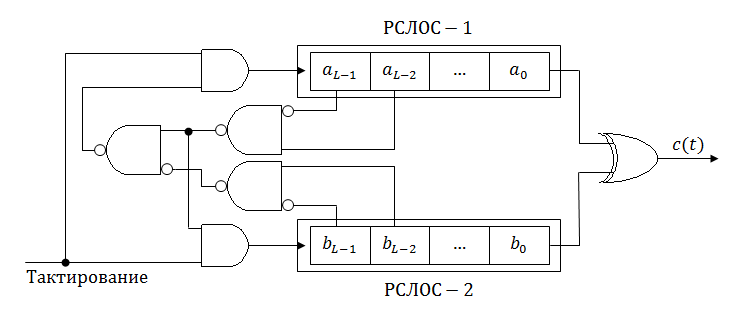
\includegraphics[scale=0.6]{stopandgo.png}}
        \caption{Схема двухстороннего генератора «старт-стоп»}
    \end{flushleft}
\end{figure}


\section{Особенности имплементации}
Программа может работать в режиме шифрования и режиме дешифрования.
На вход программе подаются следующие аргументы. 
\begin{enumerate}
	\item Тип работы программы (-e -- шифрование, -d -- дешифрование)
	\item Ключ
	\item Путь к файлу для преобразования 
\end{enumerate} 

Ключ шифрования/дешифрования прибавляется к начальным значениям регистров. \\

Для шифрования вызывается функция cipherFile класса Generator. В ней тактируются РСЛОС с помощью функции doTact.
\begin{figure}[H]
    \begin{flushleft} \centerline{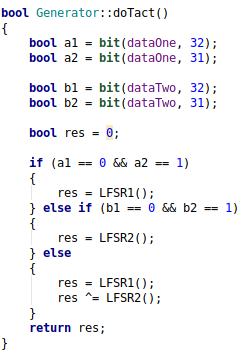
\includegraphics[scale=0.7]{dotact.png}}
        \caption{Функция, отвечающая за логику тактирования регистров}
    \end{flushleft}
\end{figure}

\section{Примеры работы программы}

\begin{figure}[H]
    \begin{flushleft} \centerline{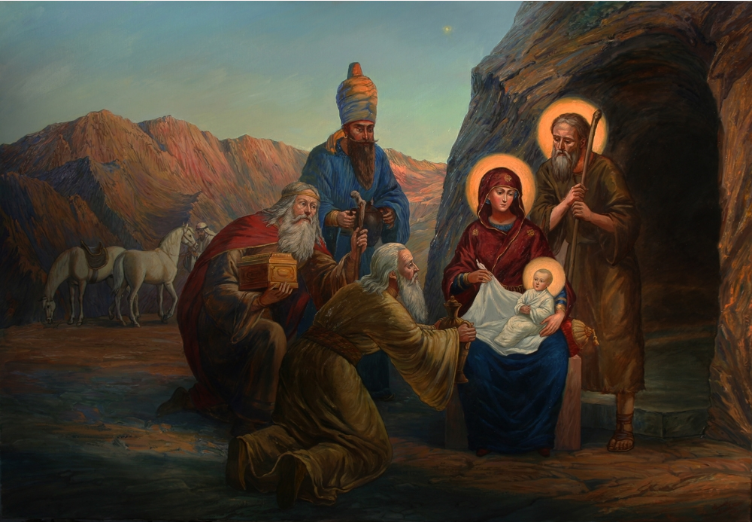
\includegraphics[scale=0.5]{openimage.png}}
        \caption{Исходное изображение}
    \end{flushleft}
\end{figure}

\begin{figure}[H]
    \begin{flushleft} \centerline{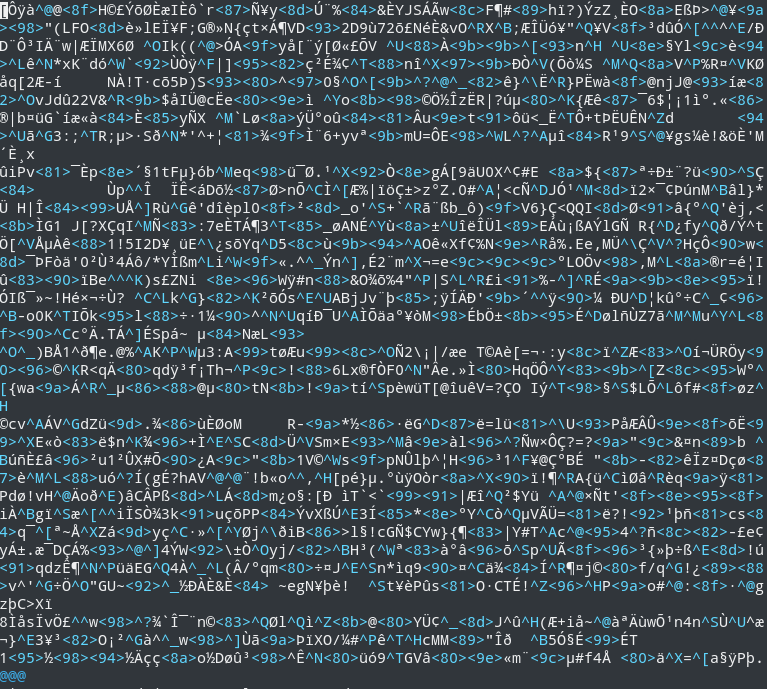
\includegraphics[scale=0.5]{cipherimage.png}}
        \caption{Зашифрованное изображение}
    \end{flushleft}
\end{figure}

\begin{figure}[H]
    \begin{flushleft} \centerline{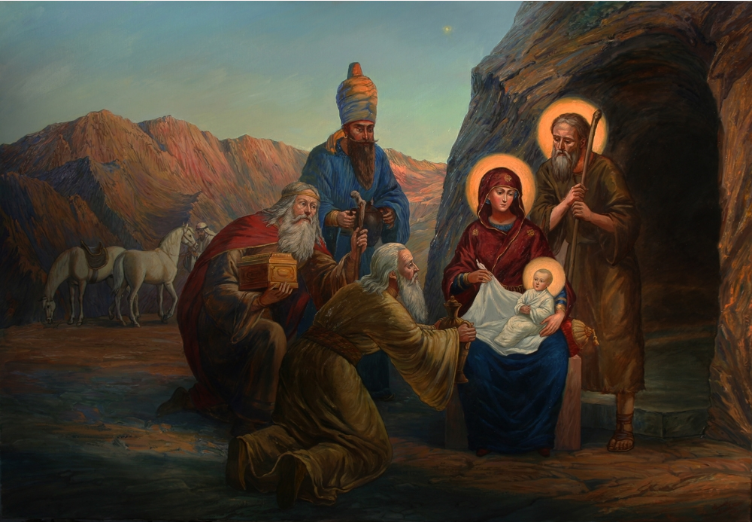
\includegraphics[scale=0.5]{openimage.png}}
        \caption{Расшифрованное изображение}
    \end{flushleft}
\end{figure}
\newpage

\section{Тестирование криптогенератора}
\begin{enumerate}
\item \textbf{Частотный тест}

Суть данного теста заключается в определении соотношения между нулями и единицами во всей двоичной последовательности. Цель — выяснить, действительно ли число нулей и единиц в последовательности приблизительно одинаковы, как это можно было бы предположить в случае истинно случайной бинарной последовательности.

\begin{figure}[H]
    \begin{flushleft} \centerline{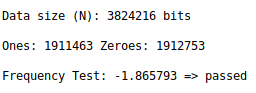
\includegraphics[scale=0.7]{freqtest.png}}
        \caption{Результат частотного теста}
    \end{flushleft}
\end{figure}

Данный тест был пройден, так как значение теста лежит в интервале от -3 до 3.

\item \textbf{Тест последовательностей}

В последовательном тесте с параметром L, последовательность длины N нарезается на N/L последовательных блоков длины L, и определяется число появлений двоичного представления целого числа. Затем определяется статистика теста.
L = 8
\begin{figure}[H]
    \begin{flushleft} \centerline{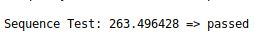
\includegraphics[scale=0.7]{seqtest.png}}
        \caption{Результат теста последовательностей}
    \end{flushleft}
\end{figure}

Данный тест был пройден, так как значение теста меньше чем квантиль хи квадрат для $2^8$ равный 284.3359

\item \textbf{Тест серий}

Суть состоит в подсчёте полного числа серий в исходной последовательности, где под словом «серия» подразумевается непрерывная подпоследовательность одинаковых битов. Цель данного теста — сделать вывод о том, действительно ли количество серий, состоящих из единиц и нулей с различными длинами, соответствует их количеству в случайной последовательности. В частности, определяется быстро либо медленно чередуются единицы и нули в исходной последовательности.
L = 15
\begin{figure}[H]
    \begin{flushleft} \centerline{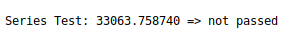
\includegraphics[scale=0.7]{seriestest.png}}
        \caption{Результат теста серий}
    \end{flushleft}
\end{figure}

Данный тест не был пройден, так как значение теста значительно больше чем квантиль хи квадрат для $2L$ равный 40.2560 
\newpage

\item \textbf{Автокорреляционный тест}

Для исходной последовательности $S^N$ автокорреляционным тестом с задержкой T называют частотный тест для последовательности $S_1\oplus S_{1+T}$, $S_2\oplus S_{2+T}$, ... , $S_{N-T}\oplus S_{T}$ где $\oplus$ означает сложение по модулю 2. Данный тест используется для выявления возможных корреляций между битами последовательности на расстоянии T.

\begin{figure}[H]
    \begin{flushleft} \centerline{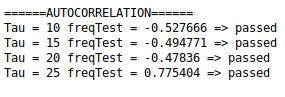
\includegraphics[scale=0.7]{autotest.png}}
        \caption{Результат автокорреляционного теста}
    \end{flushleft}
\end{figure}
Данный тест был пройден, так как значения для всех $\tau$ теста лежат в интервале от -3 до 3.

\item \textbf{Универсальный тест}
Тест оценивает, насколько «далеко» друг от друга отстоят шаблоны внутри последовательности. Смысл теста в том, чтобы понять, насколько последовательность сжимаема без потерь. Чем более сжимаема последовательность, тем она менее случайна.
\begin{figure}[H]
    \begin{flushleft} \centerline{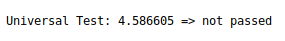
\includegraphics[scale=0.7]{unitest.png}}
        \caption{Результат универсального теста}
    \end{flushleft}
\end{figure}

Данный тест не был пройден, так как не принадлежит интервалу от -1.9 до 1.9. 

\end{enumerate}

\section{Вывод}

В ходе лабораторной работы была реализована потоковая система шифрования при помощи двухстороннего генератора «старт-стоп». 

Был проведен анализ криптостойкости криптогенератора. Два из пяти тестов не были пройдены, следовательно данный генератор нельзя назвать криптостойким при больших N.

\end{document}
